%% Manuscript for Government Information Quarterly (Elsevier), research article.
%% Double anonymized review: this file carries no author information; the
%% authors, CRediT roles and declarations are in title-page.tex. Set
%% \anonymousfalse for the preprint and the accepted version.
%%
%% Every number comes from ../study/results.json, written by
%% ../study/measure.py; the figures are drawn by the same script.
\documentclass[review,authoryear,12pt]{elsarticle}

\usepackage[T1]{fontenc}
\usepackage[utf8]{inputenc}
\usepackage{lmodern}
\usepackage{microtype}
\usepackage{amsmath}
\usepackage{booktabs}
\usepackage{tabularx}
\usepackage{graphicx}
\usepackage{xcolor}
\usepackage{lineno}
\usepackage[hyphens]{url}
\usepackage[colorlinks=true,allcolors=blue!50!black]{hyperref}

\graphicspath{{../study/figures/}}
\linenumbers

\newif\ifanonymous
\anonymoustrue

% The library and the repository of the study identify the author.
\ifanonymous
  \newcommand{\library}{the reference library}
  \newcommand{\Library}{The reference library}
  \newcommand{\repository}{an anonymized repository (link provided to the editor)}
\else
  \newcommand{\library}{\texttt{aiodpc}}
  \newcommand{\Library}{\texttt{aiodpc}}
  \newcommand{\repository}{\url{https://github.com/webysther/aiodpc}}
\fi

% U+FFFD, the replacement character, which pdfLaTeX fonts lack.
\newcommand{\replaced}{\fbox{\scriptsize ?}}
\newcommand{\field}[1]{\texttt{#1}}

\journal{Government Information Quarterly}

\begin{document}

\begin{frontmatter}

\title{Early-warning bulletins as open government data: A census of the
Italian civil protection alerts and a coded data model}

\begin{abstract}
Civil protection agencies increasingly release early-warning bulletins as
open government data, yet little is known about how well these releases serve
reuse. This study examines the national bulletins of the Italian Civil
Protection Department, released as GeoJSON files under an open licence for
every day since January 2020. Following design science research and the
ISO/IEC 25012 data quality model, it combines a census of the 2,572
criticality bulletins issued up to November 2026, including the zone
geometry of 2,571 files (15.2~GB), with a purposive sample of 73 files and a
full day of both bulletins. Zone geometry makes up 96.3\% of a criticality
file and was identical between consecutive bulletins in 99.9\% of 435,235
comparisons: a versioned reference of the zones would have changed 14 times in
almost seven years. Every alert value belongs to a small closed set of Italian
texts. The census also dates defects that a sample does not reveal:
characters lost to encoding errors in every bulletin, municipality lists that
accumulated up to 748,705 repeated names, bulletins without municipalities,
and zones renamed without stable identifiers. As its artefact, the study
proposes a coded data model, made of a versioned reference of the zones and
a small JSON document of numeric codes for each bulletin, and demonstrates it
in an open-source client library. One day of both bulletins shrinks from
19.3~MB to 15.3~kB, a quarter of bulletins from 1.83~GB to 1.1~MB, and every
value can be rendered in any language. The findings inform
publishers of warning data and the implementation of high-value dataset
obligations.
\end{abstract}

\begin{keyword}
Open government data \sep Data quality \sep Early warning \sep Civil
protection \sep Design science research \sep ISO/IEC 25012
\end{keyword}

\end{frontmatter}

%% ---------------------------------------------------------------------------
\section{Introduction}
\label{sec:introduction}

Early warnings are among the most effective measures to reduce the losses
caused by natural hazards, provided they reach the people at risk in a form
they can act upon \citep{basher2006}. The Sendai Framework for Disaster Risk
Reduction sets the target of substantially increasing the availability of and
access to multi-hazard early warning systems and disaster risk information by
2030 \citep{unisdr2015}. Next to the official channels, access is also
mediated by third parties (newsrooms, municipal portals, mobile applications,
home automation systems) that build on warnings released as open government
data. For those reusers, the value of a warning depends not only on
its scientific content but on the quality and usability of the data that carry
it.

Research on open government data has long established that the expected
benefits of openness depend on the quality of what is released and on the
effort that reuse requires \citep{janssen2012,zuiderwijk2014,safarov2017}.
Quality assessments, however, have concentrated on open data portals and their
metadata \citep{umbrich2015,neumaier2016,kubler2018,machova2017}, or on
snapshots of datasets measured along generic quality dimensions
\citep{vetro2016}. Operational datasets that are released every day, such as
warning bulletins, raise different questions: how much of each release is new
information, how stable the reference data embedded in it are, and which
defects appear, persist or disappear across releases. Answering them requires
measuring the content of every release, not a sample of it.

The question has a policy dimension. In the European Union, the Open Data
Directive asks public sector bodies to make their documents available, where
possible and appropriate, in open and machine-readable formats
\citep{eu2019opendata}, and its implementing regulation lists weather warnings
among the meteorological high-value datasets \citep{eu2023hvd}. How warning data are modelled therefore
affects the cost of complying with these obligations as well as the cost of
reusing the data.

This study examines the national bulletins of the Italian Civil Protection
Department (Dipartimento della Protezione Civile, DPC): the criticality
bulletin, which assigns an alert level to each alert zone for hydraulic,
thunderstorm and hydrogeological risk, and the national weather vigilance
bulletin. DPC releases both every day as GeoJSON files, under the CC BY 4.0
licence, in two public repositories
\citep{dpc2026criticality,dpc2026vigilance}. The study addresses three
research questions:

\begin{description}
\item[RQ1] What do the files of the bulletins contain, and how much of their
content changes from one bulletin to the next?
\item[RQ2] Which data quality defects do the files present, classified by the
characteristics of ISO/IEC 25012, and when did they occur?
\item[RQ3] Can a coded data model carry the same information, and what does it
save for publishers and reusers?
\end{description}

The study makes three contributions. First, it provides a longitudinal,
content-level quality assessment of an operational warning dataset, based on a
census of every bulletin released over almost seven years rather than on a
sample. Second, following design science research
\citep{hevner2004,peffers2007}, it proposes and evaluates an artefact: a coded
data model that separates the static reference of the zones from the daily
alerts, demonstrated by an open-source implementation. Third, it shows that a
census of this size is feasible with modest means, by reducing every file to
digests while it is downloaded, and it reports how the census corrected the
findings of a sample.

The remainder of the paper is organised as follows.
Section~\ref{sec:background} reviews the related work and the Italian alert
system. Section~\ref{sec:method} presents the research design.
Section~\ref{sec:results} reports the results for RQ1 and RQ2, and
Section~\ref{sec:artefact} presents and evaluates the artefact (RQ3).
Section~\ref{sec:discussion} discusses the implications and the threats to
validity, and Section~\ref{sec:conclusion} concludes.

%% ---------------------------------------------------------------------------
\section{Background and related work}
\label{sec:background}

\subsection{The quality of open government data}

Data quality is commonly understood as fitness for use by data consumers,
along multiple dimensions such as accuracy, completeness, consistency and
accessibility \citep{wang1996}. Assessment methodologies combine subjective
and objective measures \citep{pipino2002} and differ in the phases,
dimensions and techniques they cover \citep{batini2009}. ISO/IEC 25012 defines
a data quality model of fifteen characteristics, classified as inherent to the
data or dependent on the system that holds them \citep{iso25012}, and ISO/IEC
25024 defines quality measures for them \citep{iso25024}. The Italian
guidelines on open data recommend this model to public administrations
\citep[section 5.3]{agid2023}.

For open government data, \citet{vetro2016} defined a measurement framework
and applied it to Italian datasets. A second line of work assesses open data
portals and their metadata, automatically and over time
\citep{umbrich2015,neumaier2016}, comparing portals with multi-criteria
methods \citep{kubler2018} or at the national level \citep{machova2017}.
Systematic reviews describe the initiatives and their stages
\citep{attard2015}, and the types, conditions, effects and users of open data
utilisation \citep{safarov2017}. Data quality recurs as a condition of
utilisation and a barrier to adoption \citep{janssen2012,safarov2017}. Most
assessments, however, measure metadata, or the content of a dataset at one
point in time. Few follow the content of a frequently released dataset across
all its releases, which is where defects of operational processes become
visible.

\subsection{Standards for publishing data and warnings}

The W3C Data on the Web Best Practices recommend, among others, persistent
identifiers, versioned data, standardised vocabularies and metadata that
describe the structure of the data \citep{loscio2017}. JSON, the syntax of
GeoJSON, is an Internet standard \citep{bray2017}, and the structure of a JSON
document can be described by JSON Schema \citep{pezoa2016}. The FAIR principles
ask for globally unique and persistent identifiers, rich metadata and the use
of shared vocabularies, so that data are findable, accessible, interoperable
and reusable \citep{wilkinson2016}. GeoJSON, the format of the DPC files, notes
that six decimal places of a coordinate are about 10~cm
\citep[section 11.2]{butler2016}.

The Common Alerting Protocol (CAP) is the established format for exchanging
all-hazard alerts and public warnings, each message describing one alert and
its areas by polygons, circles or geocodes \citep{westfall2010}. CAP serves the
dissemination of individual messages. The bulletins studied here are a
different object: a national dataset that assigns a value to every zone of the
country every day, which reusers download in bulk. The model proposed in
Section~\ref{sec:artefact} addresses this dataset view and is complementary to
CAP.

\subsection{The Italian alert system and its bulletins}

The Italian national warning system for hydrogeological and hydraulic risk is
organised by a directive of the President of the Council of Ministers of 27
February 2004 \citep{dpcm2004}. DPC issues a national criticality bulletin
every afternoon for the current and the following day, and a national weather
vigilance bulletin for three days. The criticality bulletin assigns to each
alert zone a criticality for each of three risks (hydraulic, thunderstorms and
hydrogeological), each associated with an alert colour. The vigilance bulletin
gives the expected precipitation of each vigilance zone and the significant
weather phenomena as points. Two public repositories, created in April 2021,
hold the files of both bulletins for every day since 1 January 2020 in several
formats (GeoJSON, TopoJSON, shapefile, XML, PDF and images)
\citep{dpc2026criticality,dpc2026vigilance}.

%% ---------------------------------------------------------------------------
\section{Research design}
\label{sec:method}

\subsection{Design science research}

The study follows design science research, which builds an artefact to address
a relevant problem and evaluates it rigorously \citep{hevner2004}, in the six
activities of the design science research methodology \citep{peffers2007}
(Table~\ref{tab:dsr}). The artefact is a data model with its implementation;
in the knowledge contribution framework of \citet{gregor2013}, the study is an
improvement, a new solution to a known problem.

\begin{table}[t]
\centering
\caption{Activities of the design science research methodology
\citep{peffers2007} in this study.}
\label{tab:dsr}
\small
\begin{tabularx}{\linewidth}{@{}lX@{}}
\toprule
Activity & In this study \\
\midrule
Problem identification and motivation & Size, redundancy, Italian-only
texts and defects of the files (Section~\ref{sec:results}) \\
Objectives of a solution & Smaller files, values independent of language,
stable identifiers, no change for current reusers
(Section~\ref{sec:design}) \\
Design and development & A versioned reference of the zones, a daily document
of codes per bulletin and code lists, implemented in \library{}
(Section~\ref{sec:design}) \\
Demonstration & The documents of a fixed bulletin, built from the current
files, and a quarter of bulletins as JSON Lines
(Section~\ref{sec:demonstration}) \\
Evaluation & Sizes and reading times measured on a full day; the tests of the
implementation (Section~\ref{sec:evaluation}) \\
Communication & This paper, a technical report in English and Italian, the
code and the data \\
\bottomrule
\end{tabularx}
\end{table}

\subsection{Data quality model}

The defects are classified by the characteristics of ISO/IEC 25012
\citep{iso25012} and measured, where a measure applies, as in ISO/IEC 25024
\citep{iso25024}. The model extends the dimensions of \citet{wang1996}, has been
applied to Italian open government data \citep{vetro2016}, and is the model
of the Italian guidelines \citep{agid2023}, which makes its terms familiar to
the publisher.

\subsection{Data collection}
\label{sec:data}

Four sources of data were combined (Table~\ref{tab:sources}). All refer to the
bulletins issued up to 15 November 2026.

\begin{table}[t]
\centering
\caption{Sources of data. A bulletin-day is one of the two days that a
criticality bulletin covers.}
\label{tab:sources}
\small
\begin{tabularx}{\linewidth}{@{}lXl@{}}
\toprule
Source & Content & Used for \\
\midrule
Census of the summaries & The summary file of every criticality bulletin
from 1 January 2020: 2,572 bulletins on 2,511 days & RQ1, RQ2 \\
Census of the zones & The GeoJSON file of the current day of every bulletin:
2,571 files, 15.2~GB & RQ1, RQ2 \\
Purposive sample & 73 criticality GeoJSON files, 12,250 zone-days & RQ1, RQ2 \\
One full day & The eight files of 15 November 2026 & RQ1, RQ3 \\
\bottomrule
\end{tabularx}
\end{table}

The \emph{census of the summaries} reads the HTML summary that DPC publishes
with each bulletin, which states the alert headings of each day. The
\emph{census of the zones} downloads the GeoJSON file of the current day of
every bulletin and reduces each file, as it arrives, to a digest of the shape
and of the set of municipalities of each zone, and to counts of damaged and
repeated names; no file is stored. One bulletin, issued on 29 September 2020,
has no GeoJSON file. The \emph{purposive sample} was drawn at random (seed~7),
25 bulletin-days from each of three strata chosen for the variety of their
texts: days with a red alert (206 bulletin-days in the census of the
summaries), with an orange alert (1,052) and with several risks at the same
level (2,854); the strata overlap, which yields 73 files. Purposive sampling
selects the cases that best inform a question and does not represent the
population \citep{etikan2016}; the sample is therefore used for the texts of
the zones, and the census for every claim about frequency and time. The
\emph{full day} consists of the two criticality files (current and following
day), the three vigilance files and the three phenomena files of 15 November
2026 (criticality bulletin \field{20261115\_1421}, vigilance bulletin
\field{20261115}).

Two findings were triangulated \citep{denzin1978}: the closed set of alert
texts is found both in the summaries and in the zones of the sample, and the
encoding defect is measured in the files and was reported independently on the
DPC repository \citep{dpc2024issue10}.

\subsection{Measurement}

Sizes are the bytes of the files as published, raw and compressed with gzip.
The composition of a file is measured by serialising the geometry, the
municipality lists and the remaining properties of its features separately.
Two shapes are considered equal when the SHA-256 digests of their JSON
serialisation with sorted keys are equal; 64 bits of each digest are kept, so
that a collision among a few thousand shapes is negligible. The same applies to
the set of municipalities of a zone, after removing repeated names. A
\emph{change} is a difference between a bulletin and the previous one. A change
that the next bulletin undoes exactly is classified as a defect of that
bulletin, not as a change of the zones. A \emph{version} of the reference is a
state of the names, shapes and municipality sets of the zones that starts with
a lasting change. A name has a \emph{lost character} when a question mark
stands between two letters (``Valle d?Aosta''), and a \emph{replaced
character} when it contains the Unicode replacement character U+FFFD. The
repeated names of a zone are the entries of its list beyond the distinct ones.
Reading times are the fastest of five runs on one machine and are reported
only as orders of magnitude.

\subsection{Reproducibility}

The study follows the rules of reproducible computational research
\citep{sandve2013,peng2011}. A single script performs every download,
measurement and figure and writes every number reported here to one results
file; the inputs (the last day measured, the bulletin of the full day, the
seed of the sample) are constants of the script; nothing is edited by hand
between the data and the figures. The census keeps its digests in a cache, so
that a second run reads only new bulletins. Its method was first validated on
the bulletins from 9 November 2025 to 18 January 2026, against the sampled
files of that period and against a direct comparison of the shapes, without
digests. The code, the results and the tests are available in
\repository{}.

%% ---------------------------------------------------------------------------
\section{Results}
\label{sec:results}

\subsection{What is published (RQ1)}

Table~\ref{tab:day} lists the GeoJSON files of one day. The two bulletins
amount to 19.3~MB a day (7.6~MB compressed). The 2,572 criticality bulletins
of the census were issued on 2,511 days: on 58 days DPC issued an update. The
two repositories, which also hold the other formats, weighed 6.6~GB and
12.9~GB on 16 November 2026.

\begin{table}[t]
\centering
\caption{The GeoJSON files of one day of both bulletins (15 November 2026).}
\label{tab:day}
\small
\begin{tabular}{@{}llrr@{}}
\toprule
Bulletin & Files & Size & Features \\
\midrule
Criticality & current day, next day & 2 $\times$ 5.53~MB & 187 alert zones \\
Vigilance, zones & three days & 3 $\times$ 2.72~MB & 71 vigilance zones \\
Vigilance, phenomena & three days & 20 to 29~kB & 63 to 91 points \\
\midrule
One day & 8 files & 19.3~MB & \\
\bottomrule
\end{tabular}
\end{table}

Each zone of a criticality file carries its name (\field{Nome zona}), its
municipalities by name (\field{Comuni}), its shape and four texts: the
summary shown on the map and one assessment for each risk, such as
\field{Ordinaria / ALLERTA GIALLA}. A vigilance zone carries its name
(\field{Nome\_Zona}), its municipalities (\field{comuni}), its shape, the class
of expected precipitation (\field{id\_classificazione}, a number) and its text.
A phenomenon is a point with a numeric code (\field{id\_fenomeno}).

\subsection{What the files are made of (RQ1)}

The alerts themselves occupy a small part of each file
(Fig.~\ref{fig:composition}, Table~\ref{tab:composition}). In a criticality
file, 96.3\% of the bytes are the shapes of the zones, 2.1\% the municipality
lists and 1.4\% the names and the alerts. The phenomena files are small
already. The coordinates of the criticality shapes have up to 15 decimals and
those of the vigilance up to 8; rounded to the six decimals that the GeoJSON
specification considers about 10~cm \citep{butler2016}, the criticality shapes
would be 44.4\% smaller and the shapes of a day 32.3\% smaller (12.4~MB instead
of 18.3~MB), without any change of format.

\begin{table}[t]
\centering
\caption{Share of the bytes of a zone file by content (15 November 2026).}
\label{tab:composition}
\small
\begin{tabular}{@{}lrrr@{}}
\toprule
File & Zone shapes & Municipality lists & Names and alerts \\
\midrule
Criticality & 96.3\% & 2.1\% & 1.4\% \\
Vigilance, zones & 93.8\% & 5.6\% & 0.3\% \\
\bottomrule
\end{tabular}
\end{table}

\begin{figure}[t]
\centering
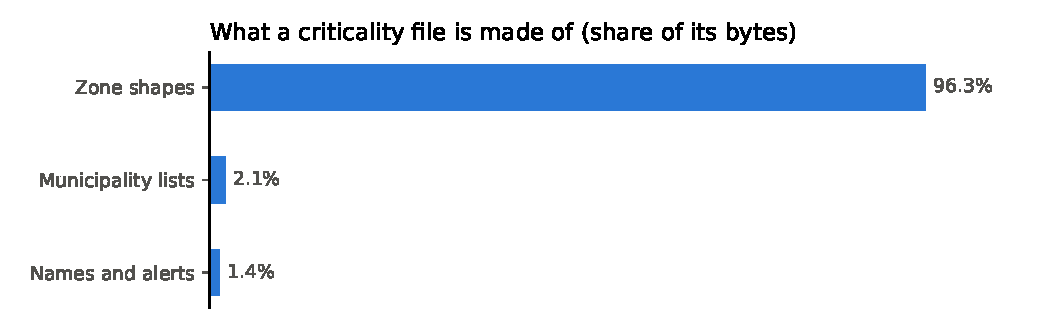
\includegraphics[width=0.85\linewidth]{en-composition.pdf}
\caption{Composition of the files of one day: the alerts are a small fraction
of the bytes.}
\label{fig:composition}
\end{figure}

\subsection{How the zones change over time (RQ1)}

The census compared the zones of each bulletin with those of the previous one
(Fig.~\ref{fig:zones}, Table~\ref{tab:versions}). Of 435,235 comparisons of a
zone with the same zone in the previous bulletin, 434,860 (99.9\%) found the
same shape. The shapes changed for good in eight bulletins. The set of zones
changed five times: one zone was renamed in February 2020, the zones grew from
158 to 168 in December 2020 and to 170 in May 2021, four zones were renamed in
May 2023, and the zones became 187 in June 2026. Zones are renamed without an
identifier that persists: ``Nodo idraulico di Milano'' became ``Nodo Idraulico
di Milano'' (a capital letter) on 15 May 2021, and ``Pianura bolognese di Reno
e suoi affluenti'' became ``Pianura bolognese'' on 23 May 2023. A reuser that
matches zones by name loses them at each change.

\begin{figure}[t]
\centering
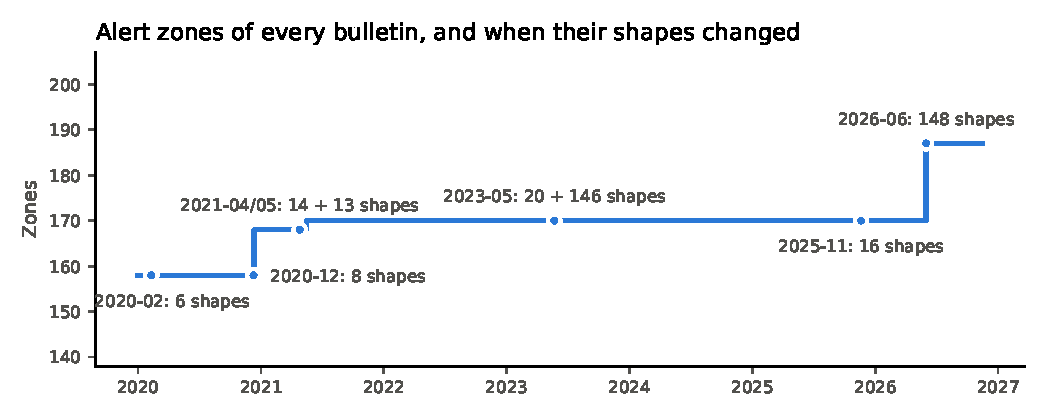
\includegraphics[width=\linewidth]{en-zones.pdf}
\caption{Number of alert zones in each of the 2,571 bulletins, and the
lasting changes of their shapes. Changes less than 90 days apart share a
label.}
\label{fig:zones}
\end{figure}

Counting every lasting change of the names, the shapes and the municipality
sets, the zones of the 2,571 bulletins come in 15 versions
(Table~\ref{tab:versions}). One of the 14 changes is caused only by the
encoding defect discussed below reaching the municipality names (8 May 2024).
Some bulletins break and the next one repairs them: on 11 May 2023, two zones
of Sicily changed shape for a single bulletin and were restored the following
day.

\begin{table}[t]
\centering
\caption{The 14 lasting changes of the zones in the census, 1 January 2020 to
15 November 2026. Names: zones added and removed (a rename counts as one of
each); shapes and municipalities: zones whose shape or set of municipalities
changed.}
\label{tab:versions}
\small
\begin{tabular}{@{}lrlrr@{}}
\toprule
Bulletin & Zones & Names & Shapes & Municipalities \\
\midrule
10 Feb 2020 & 158 & +1 / $-$1 & 6 & 17 \\
1 Apr 2020 & 158 & & & 21 \\
10 Dec 2020 & 158 & & 8 & \\
11 Dec 2020 & 168 & +18 / $-$8 & & 10 \\
1 Jan 2021 & 168 & & & 11 \\
26 Apr 2021 & 168 & & 14 & \\
15 May 2021 & 170 & +3 / $-$1 & 13 & 2 \\
18 May 2021 & 170 & & & 8 \\
27 May 2021 & 170 & & & 7 \\
23 May 2023 & 170 & +4 / $-$4 & 20 & 10 \\
26 May 2023 & 170 & & 146 & \\
8 May 2024 & 170 & & & 66 \\
20 Nov 2025 & 170 & & 16 & 62 \\
1 Jun 2026 & 187 & +26 / $-$9 & 148 & \\
\bottomrule
\end{tabular}
\end{table}

\subsection{The values of the bulletins (RQ1)}

The summaries of all 2,572 bulletins and every zone of the sample use only
the texts of Table~\ref{tab:values}. Each criticality always goes with the
same alert level: these four pairs are the only ones in the 12,250 zone-days
of the sample. The summary of a zone names a single risk, the one its map
shows, even when other risks have the same level, and no red alert for
thunderstorms was issued in the period. The precipitation of the vigilance
bulletin is already a class from 1 to 5 and the phenomena already have
numeric codes. Values that always belong to a small set are codes written in
words, in one language.

\begin{table}[t]
\centering
\caption{The closed set of criticality texts and alert levels, 2020--2026.}
\label{tab:values}
\small
\begin{tabularx}{\linewidth}{@{}XlX@{}}
\toprule
Criticality (Italian text) & Alert level & Risks \\
\midrule
Assenza di fenomeni significativi prevedibili & green & none \\
Ordinaria & yellow & hydraulic, thunderstorms, hydrogeological \\
Moderata & orange & hydraulic, thunderstorms, hydrogeological \\
Elevata & red & hydraulic, hydrogeological \\
\bottomrule
\end{tabularx}
\end{table}

\subsection{Data quality defects (RQ2)}

Table~\ref{tab:defects} classifies the defects by ISO/IEC 25012
characteristic. Three of them deserve comment because the census dates them
and reveals their mechanism.

\emph{Encoding.} A question mark replaces a letter in two or three names of
every one of the 2,571 bulletins (``Valle d?Aosta'' for Valle d'Aosta). In
addition, every bulletin with municipalities from 8 May 2024 to 19 November
2025 (568 bulletins) replaces the accented letters of up to 158 municipality
names with U+FFFD (``F\replaced{}nis'' for Fénis). The defect was reported on
the DPC repository in October 2024 \citep{dpc2024issue10}; the bulletin of
20 November 2025 fixed the replacement characters but not the question marks.

\emph{Accumulation.} 686 of the 2,571 bulletins repeat municipality names.
Until August 2021, each bulletin added one more copy of every list (8,182 to
8,215 names) to the lists of the previous bulletin, until a bulletin started
again from a single copy; the file of 31 March 2020 holds 748,705 repeated
names and weighs 15.9~MB, the largest of the census. Since 2022 the repeats
recur in isolated bulletins, 17 to 28 a year until 2025 and 7 in 2026, each
with one to seven extra copies of the lists (8,182 to 57,309 names). This
pattern is consistent with lists that are appended to rather than rebuilt when
a bulletin is produced.

\emph{Missing municipalities.} Six bulletins have no municipality list in any
zone (9 April, 5 May, 11 May and 31 October 2023, 11 March 2024 and 26 July
2025), and three bulletins of May 2021 lack it in two zones; each time, the
next bulletin restores the lists.

\begin{table}[p]
\centering
\caption{Data quality defects of the criticality and vigilance files,
classified by ISO/IEC 25012 characteristic.}
\label{tab:defects}
\footnotesize
\begin{tabularx}{\linewidth}{@{}p{2.1cm}p{3.2cm}X@{}}
\toprule
Characteristic & Defect & Evidence \\
\midrule
Accuracy & Characters lost by encoding errors & ``?'' for a letter in all
2,571 bulletins; U+FFFD in up to 158 municipality names in 568 bulletins
(8 May 2024 to 19 November 2025) \\
Accuracy & A zone name cut short & Since 1 June 2026, ``\ldots Valle di
Champorcher e Valle di Gressoney'' ends in ``\ldots Valle di Gresso'': 146
characters, exactly 150 bytes with its two typographic apostrophes, which
suggests a 150-byte field \\
Accuracy & Municipalities by name only & Seven names (Peglio, Livo, Samone,
Castro, San Teodoro, Calliano, Valverde) each denote two distant
municipalities; ``Bolzano/Bozen'' in one bulletin is ``Bolzano'' in the
other \\
Consistency & Municipalities repeated & 686 bulletins; up to 748,705 repeated
names in one file (31 March 2020) \\
Consistency & Two spellings of the same field & \field{Nome zona} and
\field{Comuni} in the criticality files, \field{Nome\_Zona} and
\field{comuni} in the vigilance files \\
Consistency & Two languages in file names & \field{\_today},
\field{\_tomorrow} for the criticality files; \field{\_oggi},
\field{\_domani}, \field{\_dopodomani} for the vigilance files \\
Consistency & Transient changes & Two shapes changed for one bulletin only
(11 May 2023) \\
Completeness & Municipalities missing & No municipalities in six bulletins
(2023--2025); in two zones of three bulletins (May 2021) \\
Completeness & A bulletin without files & Bulletin \field{20200929\_1425} has
a style file only, no GeoJSON for either day \\
Completeness & An empty field & \field{id} is empty in every phenomenon of
15 November 2026 \\
Compliance & A date with a time zone & \field{data\_bollettino} is
``2026-11-15Z'', not an ISO 8601 date \\
Traceability & Zones without identifiers & Zones are identified by name only,
and renamed (Table~\ref{tab:versions}) \\
Efficiency & Static data released daily & 18.3 of the 19.3~MB of a day are
shapes that changed in 8 of 2,571 bulletins \\
Efficiency & Needless precision & Coordinates with 15 decimals; 6 are about
10~cm \\
\bottomrule
\end{tabularx}
\end{table}

%% ---------------------------------------------------------------------------
\section{The artefact: a coded data model (RQ3)}
\label{sec:artefact}

\subsection{Objectives and design}
\label{sec:design}

From the problems identified, the artefact pursues four objectives: (O1) to
release the daily information without repeating the static reference data;
(O2) to express every value independently of language; (O3) to identify zones
and municipalities by stable codes; and (O4) to leave the current files and
their reusers untouched. The model has three components, released next to the
current files.

\begin{enumerate}
\item \emph{A versioned reference of the zones.} One file of the alert zones
and one of the vigilance zones, each zone with a stable code, its name, its
shape and the ISTAT codes of its municipalities. A new version is released only
when the zones change, with the date from which it applies; previous versions
remain available.
\item \emph{A daily document of codes for each bulletin}, naming the version of
the zones it uses, with a row of codes per zone and day: criticality (day,
zone, alert level of the zone, risk shown on the map, alert level of each
risk); vigilance (day, zone, precipitation class), with the phenomena (day,
phenomenon code, latitude, longitude).
\item \emph{Code lists} for every value, with their labels in Italian, which
keep the codes DPC already uses (\field{id\_classificazione},
\field{id\_fenomeno}).
\end{enumerate}

The design follows the W3C best practices on identifiers, versioning and
vocabularies \citep{loscio2017}. The documents are JSON \citep{bray2017},
the syntax DPC already releases, and their structure can be described by a
JSON Schema \citep{pezoa2016}. Each document fits on one line, so the
documents of a period, one per line, form a JSON
Lines\footnote{\url{https://jsonlines.org}} file: the history of a bulletin
in a single file that grows by one line per release. Stable identifiers with
shared code lists support interoperability and reuse in the sense of the FAIR
principles \citep{wilkinson2016}. A separate column for the
criticality is not needed, since in every bulletin measured it follows from the
alert level (Table~\ref{tab:values}), but it can be kept for clarity.

\subsection{Demonstration}
\label{sec:demonstration}

\Library{}, an open-source Python client of the DPC bulletins, implements the
model: it builds the daily documents and the reference of the zones from the
current files, and it renders every code in 13 languages, among them Italian,
English, French, German and Spanish. Its Italian labels
reproduce every text that DPC writes, which its tests verify. Since DPC
publishes no zone codes, the implementation numbers the zones by name and marks
each set of zones with a fingerprint, a digest of their names, municipalities
and shapes, so that a reuser knows when to fetch the reference again; codes
issued by DPC would remain stable across versions. Applied to the bulletins of
15 November 2026, it yields documents such as the following (shortened), of
7.5~kB for the criticality bulletin, in which zone~28 has a green alert for
every risk on the current day:

\begin{verbatim}
{"schema":1,"kind":1,"bulletin":"20261115_1421",
 "zone_set":"68bcac32826e",
 "columns":["day","zone","level","criticality","mapped_risk",
            "hydraulic","thunderstorms","hydrogeological"],
 "rows":[[0,28,1,1,0,1,1,1],[0,39,1,1,0,1,1,1],...]}
\end{verbatim}

The same implementation wrote every bulletin of the third quarter of 2026 as
two JSON Lines files: the 97 criticality and 92 vigilance bulletins released
from 1 July to 30 September take 1.1~MB, and 101~kB compressed, against
1.83~GB in the 746 files that DPC released for them, 1,639 times less. All of
them use one set of zones of each kind, whose two references add 8.2~MB once.
The files are available with the implementation, as an example for reusers.

\subsection{Evaluation}
\label{sec:evaluation}

Table~\ref{tab:savings} and Fig.~\ref{fig:sizes} compare the files of one day
with the daily documents that carry the same values. One day of both
bulletins shrinks from 19.3~MB to 15.3~kB, 1,259 times less, and from 7.6~MB
to 4.0~kB compressed, 1,894 times less. A year of both bulletins would take
5.6~MB instead of 7.0~GB. Reading a day takes about 0.4~s from the GeoJSON
files and 0.3~ms from the documents. The reference of the zones weighs 5.3~MB (alert zones)
and 2.6~MB (vigilance zones) as GeoJSON, and 124~kB and 155~kB as tables of
names and municipalities, and it is downloaded once per version: 15 times in
the period of the census, compared with every day.

\begin{table}[t]
\centering
\caption{Bytes of the bulletins as released and as coded JSON documents.}
\label{tab:savings}
\small
\begin{tabular}{@{}lrrr@{}}
\toprule
 & GeoJSON & Coded JSON & Ratio \\
\midrule
One day & 19.3~MB & 15.3~kB & 1,259 \\
One day, gzip & 7.6~MB & 4.0~kB & 1,894 \\
One quarter (2026 Q3, 189 bulletins) & 1.83~GB & 1.1~MB & 1,639 \\
One year (365 days) & 7.0~GB & 5.6~MB & \\
Reading one day & about 0.4~s & 0.3~ms & over 1,000 \\
\bottomrule
\end{tabular}
\end{table}

\begin{figure}[t]
\centering
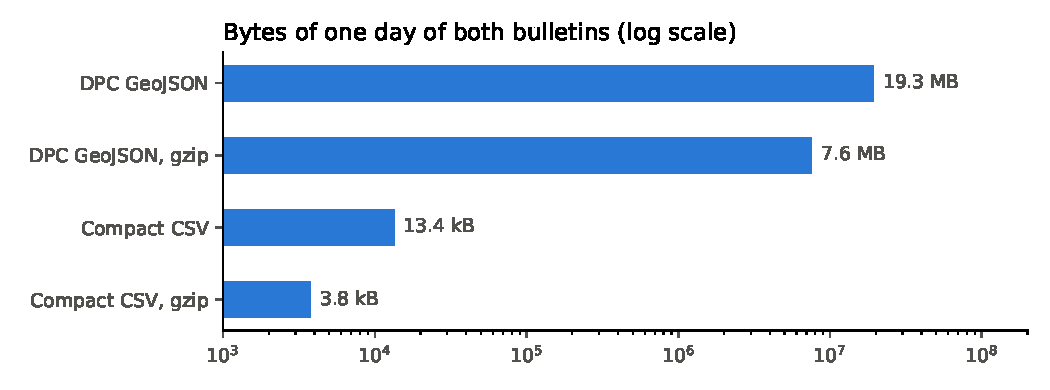
\includegraphics[width=0.85\linewidth]{en-sizes.pdf}
\caption{Bytes of one day of both bulletins, as released and as coded JSON
documents (logarithmic scale).}
\label{fig:sizes}
\end{figure}

Beyond size, the evaluation shows three further properties. Values become
independent of language: a code is rendered from a list of labels, of which
DPC's Italian texts are one. Reusers compare numbers instead of parsing
sentences whose wording varies between files. And the history of the alerts
becomes small enough to study as a whole, which today requires downloading
gigabytes.

%% ---------------------------------------------------------------------------
\section{Discussion}
\label{sec:discussion}

\subsection{Implications for publishers of warning data}

The results separate two kinds of data that the current files mix: a static
reference that changed 14 times in almost seven years, and a daily signal of a
few kilobytes. Publishing them separately is the main recommendation; it
reduces what each reuser downloads by three orders of magnitude and makes
changes of the zones explicit events, with a date, instead of differences to
be detected. Stable identifiers for zones and ISTAT codes for municipalities
remove the ambiguity of names, including homonyms and bilingual names.

The defects found by the census point to process controls rather than to
one-off corrections. Each anomalous bulletin was repaired by the next one,
which suggests faults in the production of individual releases. Simple checks
before release would have caught each of them: the presence of the
municipality lists, the absence of repeated names and of replacement
characters, and the stability of the digests of the shapes from one release
to the next. The accumulation of municipality lists went
unnoticed for months, possibly because the files remained valid GeoJSON and
displayed correctly on a map: what a map shows is not what a reuser reads.

\subsection{Implications for reusers and for policy}

For reusers, the findings quantify the cost of the current model: matching
zones by name breaks at renames, the encoding defects require ad hoc
corrections, and the size of the files excludes constrained devices from
following the alerts directly. Coded values also lower the barrier of language:
a warning can be rendered in the language of its reader from a list of
labels, rather than translated from free text.

For policy, weather warnings are a high-value dataset under the European
framework \citep{eu2023hvd}, and the Italian guidelines adopt ISO/IEC 25012
\citep{agid2023}. The study shows how that model can be operationalised for a
daily dataset: by measuring every release, dating each defect and classifying
it. It also shows that quality cannot be assessed on a sample alone. The
purposive sample placed the changes of the zones up to four and a half months
late and missed those of February 2020, before its first file; its
measurement overlooked the replacement characters, and the repeats of 2026
fell outside it. The census,
15.2~GB reduced to digests during download, was feasible on a single machine.

\subsection{Relation to prior work}

The study extends portal- and metadata-level assessments
\citep{umbrich2015,neumaier2016,kubler2018} to the content of an operational
dataset, and the dataset-level framework of \citet{vetro2016} from a snapshot
to every release over time. It complements CAP \citep{westfall2010}, which
standardises individual alert messages, with a model for the national,
bulk view of the same warnings.

\subsection{Threats to validity}

Following \citet{wohlin2012} and \citet{runeson2009}:

\emph{Construct validity.} Size is the number of bytes as released, raw and
compressed; what travels on the network depends on the server, so both are
reported. ``The same information'' means every value of the alerts and the
phenomena; the Italian texts are not kept as text, but they belong to a closed
set that the codes reproduce, as the tests of the implementation verify. Zones
are matched by name, so a renamed zone counts as one removed and one added.
Shapes are compared by digests of their serialisation: points in a different
order or with different decimals count as a change.

\emph{Internal validity.} The measures come from a script, which could be
wrong. The parsing is covered by automated tests, every number of the text is
checked against the results file, and the census method was validated on a
window of bulletins against the sampled files and a direct comparison. The
measuring corrected findings of earlier drafts: an apparent change of order of
the municipality lists was in fact the repetition of names.

\emph{External validity.} The census reads one file per bulletin, that of the
current day; the files of the following day, the history of the vigilance
bulletin and the other formats were not measured. The sample favours days with
alerts, so the frequencies of its texts do not represent all days; the closed
set of texts rests on the census of the summaries. The results describe the
files up to 15 November 2026, and DPC may change or replace them. The findings
concern one publisher; whether other warning datasets show the same pattern
of static data released daily is a question for further research.

\emph{Conclusion validity and reliability.} The results are counts and sizes
of a census, not estimates, and need no statistical inference. Anyone can
repeat them with the script and the same inputs; the reading times are the only
measure that depends on the machine.

%% ---------------------------------------------------------------------------
\section{Conclusion}
\label{sec:conclusion}

This study measured every release of the Italian national criticality
bulletin over almost seven years. Over 96\% of each file is a static reference
that changed 14 times; the alerts are a few kilobytes of values from small
closed sets; and the files show encoding, accumulation and completeness defects
that only a census could date. A coded data model, with a versioned reference
of the zones and a small daily JSON document per bulletin, carries the same
information in 1,259 times fewer bytes and in any language, without changing the current
files. Future work includes extending the census to the vigilance bulletin and
to the other formats, discussing the model with the publisher, and studying
how reusers of warning data are affected by the defects and by the model.

%% ---------------------------------------------------------------------------
\section*{Data availability}

The bulletins are released by the Dipartimento della Protezione Civile --
Presidenza del Consiglio dei Ministri under the CC BY 4.0 licence
\citep{dpc2026criticality,dpc2026vigilance}. The measurement script, its
results file, the figures, the data dictionary of the codes, the
implementation and the bulletins of the third quarter of 2026 as JSON Lines
are available in \repository{}.

\section*{Declaration of generative AI and AI-assisted technologies in the
manuscript preparation process}

During the preparation of this work the author used Claude (Anthropic) in
order to write and review the measurement code and to draft and edit the text.
After using this tool, the author reviewed and edited the content as needed
and takes full responsibility for the content of the published article.

\bibliographystyle{elsarticle-harv}
\bibliography{references}

\end{document}
